\chapter{Architettura interna}

In questo capitolo illustriamo l'architettura interna dell'Engine, cioè del
componente software predisposto alla messa in esecuzione dei programmi Blite.

Ricordiamo che nello scenario delineato avremo un Engine per locazione, o se si
vuole per nodo di rete, e su ognuno di questi componenti sarà possibile
installare o rimuovere definizioni di processi Blite. In pratica un engine
gestir\`a un insieme di definizioni, creando da queste istanze di
processi e utilizzerà l'Environment per interagire con gli altri Engine. 
Dall'environment stesso l'engine verrà notificato riguardo l'accadere di
eventi, quali l'arrivo di messaggi indirizzati alle porte delle sue definizioni.

Dal punto di vista logico relazionale abbiamo già individuato le seguenti
macro entità e relazioni

\begin{figure}[!htp]
\begin{center}
  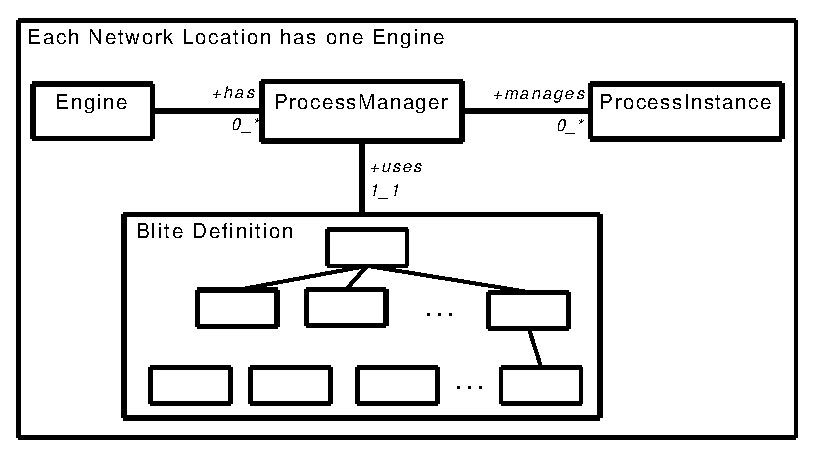
\includegraphics{architettura_interna/dia/engine}
%   \caption[]{
%   	\textsf{{\small Passaggio da reazioni a processi}}
%   }
  \label{fig:1}
\end{center}
\end{figure}

Per ogni definizione istallata sull'engine sarà presente un oggetto istanza
della classe \icode{ProcessManager}, che avrà il compito di gestire, nel loro
ciclo di vita, le istanze di processo derivate dalla definizione.

Prima di entrare nel dettaglio delle scelte architetturali ricapitoliamo quali
sono le caratteristiche peculiari di un sistema che deve gestire programmi per
l'orchestrazione di servizi, in modo che sia pi\`u facile da una parte
comprendere e dall'altra giustificare le scelte fatte.

A nostro vantaggio:
\begin{itemize}
  \item Un Engine contiene in generale un numero contenuto di definizioni, per
  cui non ci interessa la scalabilità rispetto alla quantità di definizioni
  istallate su singolo engine. Tale scalabilità al contrario può essere
  ottenuta aggiungendo altri engine e installando definizioni su engine diversi.
  
  \item  Una definizione (o programma) Blite avendo principalmente funzionalità
  di integrazione avrà una lunghezza generalmente limitata. 
  
  \item Poiché le operazione fondamentali di un programma di questo genere
  sono invocazioni remote, le durate delle esecuzioni hanno ordini di grandezza
  minimi dettati dai tempi caratteristici della rete. Per questo motivo non
  risulta determinante l'efficienza di esecuzione delle operazioni interne di un
  processo. Il nostro engine non necessiterà di una particolare ottimizzazione 
  rispetto all'efficienza di esecuzione interna.
\end{itemize}

al contrario risultano particolarmente critici i seguenti aspetti:
\begin{itemize}
  \item Per ciascuna definizione potrà essere richiesta la creazione di
  innumerevoli istanze. La scalabilità rispetto al numero delle
  richieste remote e quindi di istanze di processo risulta essere un
  prerequisito fondamentale.
  
  \item Se da un lato abbiamo detto che l'efficienza di esecuzione non \`e 
  una aspetto particolarmente critico, dall'altro per\`o ogni attività interna
  necessita di un elevato grado di controllo e tranciabilità. Ogni attività deve
  potere essere eventualmente terminata o abortita. Poiché in generale
  \footnotetext{} ogni istanza potrebbe avere un immagine persistente o
  perlomeno essere soggetta ad una attività di monitoring, l'engine necessiterà
  di un grado di controllo a livello di singola attività Blite.
\end{itemize}

Tenendo conto di queste iniziali considerazioni sono state fatte alcune scelte
basilari di organizzazione del progetto e l'architettura software \`e stata
basata sulle seguenti specifiche fondamentali:

\begin{enumerate}
  \item La compilazione di una definizione Blite (che eventualmente in un
  ambiente distribuito può essere fatta in fase di deploy) produce un modello
  statico della definizione stessa. Tale modello può essere implementato con una
  struttura ad oggetti che si può pensare di mantenere in memoria presso
  l'engine, tale struttura sarà navigata a runtime per ricavare il
  flusso e la logica di esecuzione. Sempre in fase di deploy l'engine può
  ricavare tutte le informazioni per popolare le strutture dati in cui sono 
  memorizzati i binding fra i nomi delle porte e le definizioni; anche tali
  strutture dati possono essere mantenute in memoria.
  
  \item Le richieste che giungono all'Engine non devono produrre un aumento
  delle risorse complessive mantenute dall'Engine. Ogni istanza di processo nel
  suo svolgersi deve, man mano che procede, rilasciare le risorse di memoria
  acquisite. Anche il numero dei thread complessivo deve essere limitato
  superiormente (generalmente dell'ordine dell'unita). La realizzazione del
  parallelismo di attività deve essere attuata tramite il pattern ``Resources
  Pool''. Ogni Engine deve disporre di un pool di thread con cui eseguire in
  parallelo le attività secondo le definizioni Blite.
  
  \item Il modello di esecuzione deve essere Activity Centric. L'engine deve
  trattare ogni attività secondo una astrazione generica che possa permettere di
  fattorizzare i comportamenti comuni e mantenere semplice e pulita
  l'implementazione della semantica di esecuzione del linguaggio.
\end{enumerate}

%%%%%%%%%%%%%%%%%%%%%%%%%%%%%%%%%%%%%%%%%%%%%%%%%%%%%%%%%%%%%%%%%%%%%%%%%%%%%%%%
%						Modello per l'Attività
%%%%%%%%%%%%%%%%%%%%%%%%%%%%%%%%%%%%%%%%%%%%%%%%%%%%%%%%%%%%%%%%%%%%%%%%%%%%%%%%
\section{Modello per l'Attività}
A questo punto dopo aver esposto a grandi linee quelle che devono essere le
caratteristiche fondamentali di un engine entriamo nel dettaglio del disegno
della architettura. Nella realizzazione di questa abbiamo scelto di utilizzare
il formalismo degli oggetti e delle classi secondo il consueto paradigma
``Object Oriented''. Inoltre abbiamo preso come fonte di
ispirazione il ``Composite Pattern'' [GANGo4] cercandone una trasposizione nella
problematica dell'esecuzione di un programma Blite. In particolare
l'astrazione di componente \`e stata applicata all'entità attività. Come i
componenti contribuiscono alla realizzazione di un documento o di una
interfaccia utente le singole attività contribuiscono allo svolgersi
dell'esecuzione del processo Blite.
 
Inoltre la tipica struttura gerarchica presente staticamente negli elementi
sintattici di una definizione può essere naturalmente riprodotta a runtime tra
i singoli step di esecuzione, andato a completare l'analogia con le strutture
gerarchiche ad albero tipiche dei tradizionali domini di applicazione del
Composite Pattern. 
\\

L'entità fondamentale del nostro dominio applicativo \`e stata quindi
individuata nella \icode{ActivityComponent} trasposizione a runtime
dell'elemento sintattico Activity definito dalla grammatica di Blite.
Ogni \icode{ActivityComponent} \`e rappresentabile tramite la seguente
interfaccia

\lstinputlisting
[caption={L'interfaccia base del modello di escuzione del Blite Engine},
label=lst:ActivityComponent]
{architettura_interna/java/ActivityComponent.java}

\begin{tabular}{| p{0.3\textwidth } | p{0.6\textwidth}|}
\hline
\icode{ActivityComponent} &  \\
\hline

\small{boolean \textbf{doActivity()}} & \small{\textsf{Costituisce il metodo
centrale per lo svolgersi dell'esecuzione del programma. L'invocazione di tale metodo su
un oggetto attività fa si che essa possa eseguirsi. Il valore booleano
ritornato sarà il discriminate del fatto che il flusso di esecuzione
corrente dovrà o meno interrompersi. Ogni attività oltre che eseguire se
stesa sarà quindi anche responsabile nel guidare il flusso nel passo
successivo. Utilizzando la gerarchia a lei nota imposterà la nuova attività
corrente da eseguire (l'attività padre o un figlio) e ritornerà il valore true. 
Al contraio potrà interrompere il flusso corrente ritornando false.
}}\\
 
& \\
\small{ActivityComponent \linebreak \textbf{getParentComponent()}} &
\small{\textsf{ Tale metodo restituisce se presente l'elemento padre 
dell'attività corrente. In questo modo si realizza la struttura gerarchica fra
i veri componenti dell'esecuzione. }}\\

& \\
\small{BltDefBaseNode \linebreak {\textbf{ getBltDefNode()}}} &
\small{\textsf{ Ogni attività componente dell'esecuzione \`e strettamente 
associata ad un elemento sintattico del programma. Con questo metodo ogni 
oggetto attività restituisce il nodo che la definisce nell'albero sintattico
ricavato dal parsing del codice Blite. }}\\

\hline
\end{tabular}


Lo scenario che si va a delineare \`e quindi quello di due strutture gerarchiche
associate: una costituita dall'AST (Abstract Syntax Tree) ricavato dal
parsing del codice Blite, e che come si detto \`e mantenuta nella sua interezza,
l'altra costituita dall'albero dinamico delle ActivityComponent che
realizzano l'esecuzione a runtime. Quest'ultima struttura, una per ogni
istanza, non \`e pero costruita in un unico momento in fase di inizializzazione
del  processo, ma al contrario \`e istanziata man mano che l'esecuzione
procede.  Come già accennato le attività stesse saranno responsabili di creare
i loro successori e di metterli in esecuzione. Inoltre gli oggetti attività
già eseguiti dovranno essere rilasciati il prima possibile in modo da poter 
essere collezionati dal Garbage Collector e rilasciare le risorse di memoria.

\begin{figure}[!htp]
\begin{center}
  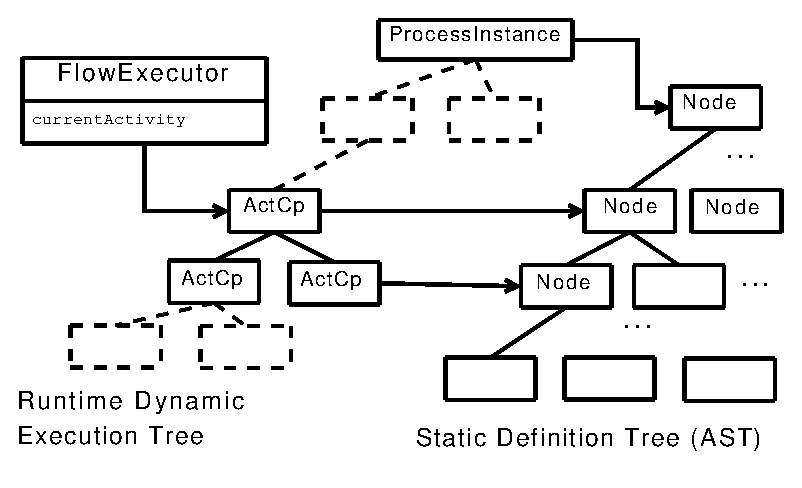
\includegraphics{architettura_interna/dia/tries}
%   \caption[]{
%   	\textsf{{\small Passaggio da reazioni a processi}}
%   }riscrivera
  \label{fig:1}
\end{center}
\end{figure}

Per ogni tipologia di attività prevista dalla grammatica di Blite esisterà
una sotto classe specifica implementante l'interfaccia \icode{ActivityComponent}
e che realizzerà in maniera opportuna, in rispetto della semantica, il metodo
\icode{boolean \textbf{doActivity()}}. Per ottimizzare il disegno e fattorizzare
il codice comune \`e stata ovviamente introdotta una classe astratta
\icode{ActivityComponentBase} da cui ogni altra implementazione di
\icode{ActivityComponent} erediterà le funzionalità comuni di base.

Anche la classe \icode{ProcessInstance}, che modellerà con i suoi oggetti le
varie istanze di processo nell'engine, implementerà l'interfaccia
\icode{ActivityComponent} uniformando la struttura gerarchica di esecuzione.

Le varie istanze di \icode{ActivityComponent} del tipo specializzato verranno
create tramite una classe di Factory \icode{ActivityComponentFactory} che
espone il FactotyMathod \icode{ActivityComponent
\textbf{makeRuntimeActivity}(BltDefBaseNode bltDefNode,\ldots )} 

\lstinputlisting
[caption={ActivityComponentFactory la factory per le ActivityComponent},
label=lst:ActivityComponentFactory]
{architettura_interna/java/ActivityComponentFactory.java}

\begin{center}
\begin{tabular}{| p{0.5\textwidth } | p{0.4\textwidth}|}
\hline
\icode{ActivityComponentFactory} & \\
\hline

\small{
ActivityComponent \linebreak \textbf{makeRuntimeActivity}( 
\linebreak \hspace*{\stretch{3}} BltDefBaseNode bltDefNode, 
\linebreak \hspace*{\stretch{3}} ExecutionContext context, 
\linebreak \hspace*{\stretch{3}} ActivityComponent parentComponent, 
\linebreak \hspace*{\stretch{3}} FlowExecutor executor)} 
& \small{\textsf{ Permette di ottenere istanze opportune di oggetti
\icode{ActivityComponent}. Il parametro bltDefNode individua l'elemento
sintattico che definisce l'attività specifica, in pratica il nodo nel AST.
Il parametro parentComponent l'attività padre nella gerarchia di esecuzione,
mentre gli altri due parametri individuano rispettivamente il contesto di
esecuzione e l'esecutore del flusso in cui l'attività verrà creata. Tali
entità verranno descritte nelle sezioni successive}}\\
\hline
\end{tabular}
\end{center}

In Figura \ref{fig:actclass} viene riportato un diagramma di classe
abbastanza dettagliato per le entità \icode{ActivityComponent}.

\begin{figure}[p]
\begin{center}
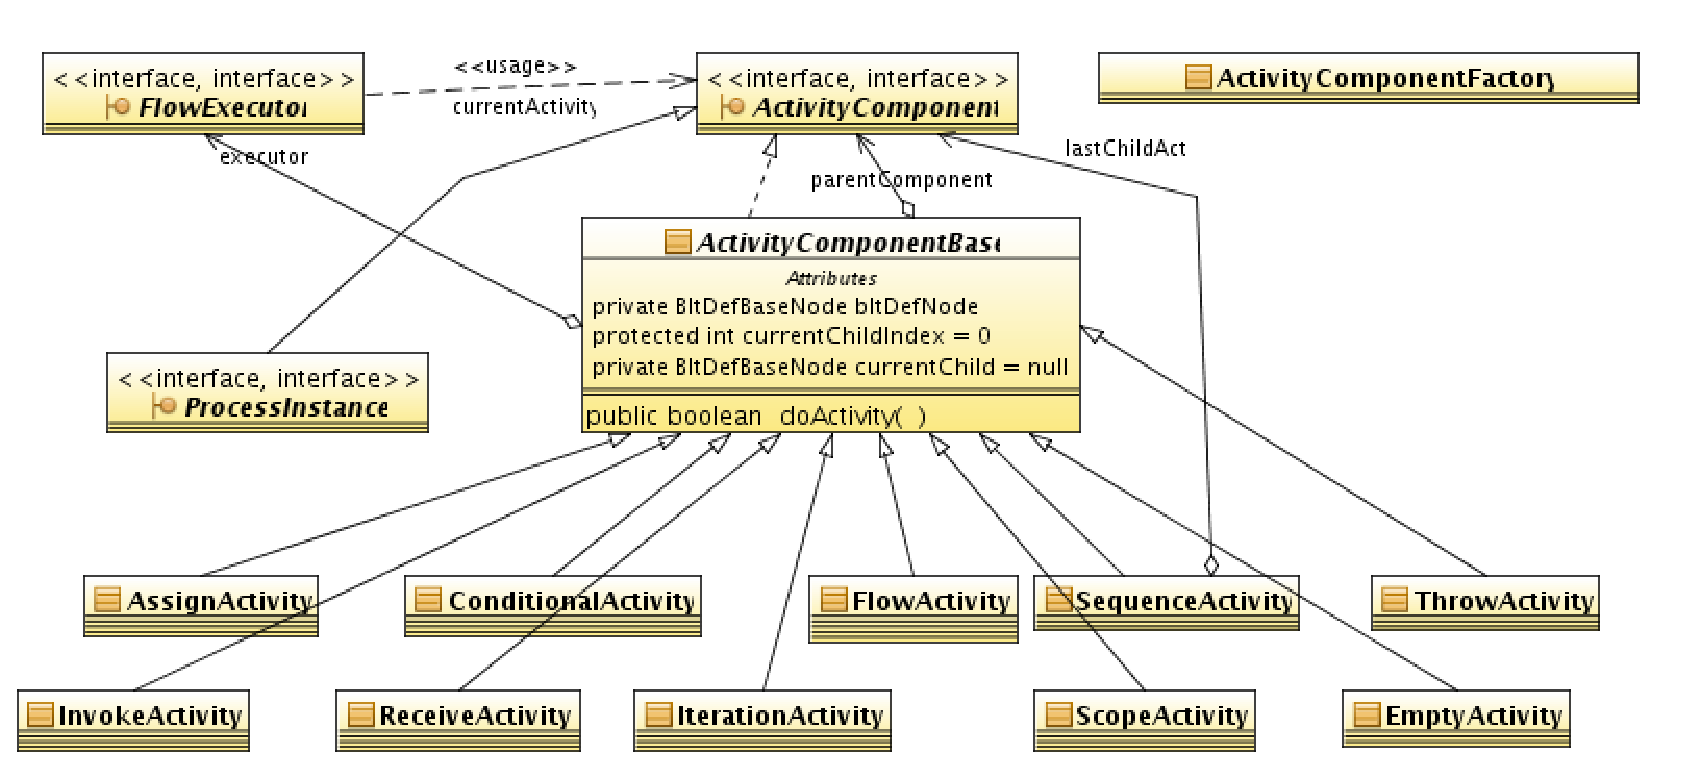
\includegraphics[angle=90,scale=0.80]
{architettura_interna/dia/actclass}
\caption[Gerarchia delle ActivityComponent]{
   	\textsf{{\small Diagramma di classe per la gerarchia delle
   	ActivityComponent}} }
  \label{fig:actclass}
\end{center}
\end{figure}

% %%%%%%%%%%%%%%%%%%%%%%%%%%%%%%%%%%%%%%%%%%%%%%%%%%%%%%%%%%%%%%%%%%%%%%%%%%%%%%%
% Esecuzione e parallelismo
% %%%%%%%%%%%%%%%%%%%%%%%%%%%%%%%%%%%%%%%%%%%%%%%%%%%%%%%%%%%%%%%%%%%%%%%%%%%%%%%
\section{Esecuzione e parallelismo}
Abbiamo visto come i componenti base per l'esecuzione siano oggetti delle varie
sottoclassi implementanti l'interfaccia \icode{ActivityComponent}, e come
l'esecuzione abbia atto tramite l'invocazione del metodo
\icode{\textbf{doActivity()}} su tali oggetti. A questo punto pero dobbiamo
domandarci da chi e in che modo tale metodo sia invocato. Nel rispondere a questa
domanda dobbiamo tenere conto che in un engine verranno eseguite
contemporaneamente molteplici istanze di processo e che inoltre il formalismo
stesso del linguaggio da la possibilità di richiedere l'esecuzione contemporanea
di diverse attività (costrutto flaw). Quindi su ciascun Engine dovranno essere
disponibili più thread per poter realizzare il sufficiente livello si
parallelismo.

Ovviamente si capisce bene che istanzire un nuovo oggetto Thread per ogni nuovo
flusso logico presente sull'engine non sia un approccio assolutamente
vantaggioso. Come già accennato infatti tale politica non sarebbe per nulla
scalabile rispetto al numero delle richieste remote gestite dell'engine; inoltre,
poiché ogni istanza di processo tendenzialmente trascorrerà la gran parte del suo
tempo in attesa di comunicazioni remote\footnote{Come già osservato i tempi di
comunicazione remota sono di ordini di grandezza molto maggiori rispetto alle
operazioni interne per cui ogni istanza nel suo ciclo di vita si troverà ad
occupare realmente la CPU per tempi quasi infinitesimi rispetto ai tempi di
attesa di eventi remoti}, ci troveremmo con un gran numero di thread in stato di
attesa, con un del tutto ingiustificabile spreco di risorse. Più banalmente
gestire direttamente oggetti Thread \`e un pratica alquanto sconsigliabile
\footnote{Questo \`e ancor pi\`u vero dalla versione 5 in poi di Java, in cui
sono stato introdotti i pacchetti \texttt{java.util.concurrent.*} che mettono a
disposizione un framework ad alto livello che ottimizza e astrae l'uso delle API
a più basso livello per la concorrenza}, in quanto può portare ad errori di
programmazione o ad Memory Leaks nel caso in cui il ciclo di vita di tali oggetti
non sia sempre ben condotto dal programmatore. Per queste motivazioni si \`e
scelto di utilizzare la tecnica del Pooling per gestire un insieme di Thread a
livello di Engine. Con tale tecnica si isola la gestione della tecnologia di
multitasking e si possono applicare politiche anche molto raffinate capaci di
adattare la quantità di risorse utilizzate al carico di lavoro da svolgere. Nella
implementazione attuale dell'Engine si \`e fatto uso dei thread pool forniti
dalla classe \texttt{java.util.concurrent.Executors} presente nella piattaforma
standard Java 5
 
La scelta che quindi \`e stata fatta per realizzare il sufficiente grado di
parallelismo \`e la seguente: ogni flusso logico attivo presente nelle varie istanze di
processo sarà associato all'entità \icode{FlowExecutor} (tale entità \`e già
comparsa in alcuni diagrammi precedentemente illustrati in questo capitolo, per
cui il lettore avrà già intuito la sua funzionalità). Tali oggetti
presenteranno un'interfaccia che permetterà da un lato di impostare l'attività corrente che
dovrà essere eseguita da uno dei thread del pool, dall'altro di eseguire
effettivamente tale attività.

\lstinputlisting
[caption={I FlowExecutors saranno gli oggetti che realizzeranno i flussi di
esecuzione parallela all'interno dell'Engine }, label=lst:FlowExecutor]
{architettura_interna/java/FlowExecutor.java}

A questo punto quando ci sarà bisogno di creare un nuovo flusso di esecuzione per
l'ActivityComponent \texttt{act} si dovrà creare un nuovo FlowExecutor settarci
\texttt{act} come attività corrente e renderlo disponibile ad un thread per
l'esecuzione. Questo ultimo passaggio verrà realizzato tramite l'interfaccia
dell'Engine che disporrà di un metodo per notificare gli executor pronti per
essere eseguiti e metterli a disposizione del pool di threads

\lstinputlisting {architettura_interna/java/queueFlowExecutor.java}

Inoltre ogni flusso giungerà a conclusione (un istanza di processo termina o un
esecuzione parallela definita in una flow Activity si conclude) e tale evento
dovrà essere registrato e produrre eventualmente altri effetti. Per far si che si
realizzi questa necessità si \`e introdotto il concetto di \icode{FlowOwner}.
Ogni attività che nel suo eseguirsi si troverà a creare nuovi flussi di
esecuzione e quindi oggetti \icode{FlowExecutor}  dovrà implementare
l'interfaccia \icode{FlowOwner} e settare se stessa nel FlowExecutor da lei
creato. In questo modo quando il flusso logico terminerà il FlowOwner potrà
essere notificato di tale accadimento tramite l'invocazione del metodo
\icode{flowCompleted()}.

\lstinputlisting
{architettura_interna/java/FlowOwner.java}

A questo punto \`e lecito domandarsi quando si dovrà considerare terminato un
flusso di esecuzione. In generale si applica il seguente ragionamento. Le varie
\icode{ActivityComponent}, che sono legate in una struttura gerarchica che
riflette la definizione statica del programma, termineranno la loro esecuzione
mettendo come attività corrente nel loro FlowExecutor la propria attività padre
(parentComponent). In accordo con questa osservazione risulta quindi corretto
affermare che flusso di esecuzione può essere considerato terminato dal
FlowExecutor quando questo si troverà ad eseguire come attività corrente proprio
il suo FlowOwner. In questo caso su di esso il FlowExecutor non dovrà invocare il
metodo doActivity() ma il metodo flowCompleted() e fatto questo, dovrà terminare
di eseguire il flusso. Il codice seguente spiega meglio di mille parole la logica
alla base di tutto il modello di esecuzione del Blite Engine; in poche righe \`e
sintetizzata il cuore dell'architettura

\lstinputlisting{architettura_interna/java/FlowExecutorImp.java}

In generale possiamo quindi dedurre le seguenti affermazioni che ci possono
aiutare a sintetizzare delle proprietà invarianti

\begin{itemize}
  \item Un FlowExecutor non invocherà mai il metodo doActivity() del suo
  FlowOwner. Viceversa di questo invocherà prima o poi il metodo
  flowCompleted().
  
  \item Su un oggetto ActivityComponent che implementa anche l'interfaccia
  FlowOwner, il metodo doActivity() verrà invocato dal FlowExecutor dell'attività 
  padre.
  
  \item Su di un oggetto ProcessInstance, che \`e il FlowOwner del flusso
  principale dell'istanza e che \`e l'unica attività senza padre, 
  il metodo doActivity() non verrà mai invocato da nessun FlowExecutor.
  
  \item il metodo doActivity() di una ProcessInstance verra' invocato
  dell'Engine stesso in fase di creazione dell'istanza.
  
\end{itemize}

Oltre a creare, eseguire e terminare flussi sarà anche necessario sospenderne
alcuni già in esecuzione, vedi per esempio il caso dell'attività di ricezione
che deve fermare il flusso corrente in attesa di un evento remoto. In questo
caso l'attività utilizzando l'interfaccia dell'Engine e in particolare il
seguente metodo

\lstinputlisting{architettura_interna/java/addFlowWaitingEvent.java}

potrà mettere in attesa il suo FlowExecutor su di un evento identificato dalla
chiave \texttt{eventKey} e che lei stessa aveva provveduto
precedentemente a creare. Fatto questo l'attività ritornerà dal proprio metodo
doActivity() con il valore false, in questo modo il FlowExecutor terminerà
l'esecuzione del Flow corrente. Nel momento in cui il messaggio sarà recapitato,
l'Engine potrà individuare il FlowExecutor tramite la chiave \texttt{eventKey} e
rimetterlo in esecuzione, poiché l'attività corrente di quest'ultimo sarà rimasta
l'attività di ricezione essa potrà riprendere il suo lavoro, consumando il
messaggio e permettendo al suo flusso di esecuzione di continuare. Nella sezione
successiva verrà illustrato nel dettaglio come si realizza la comunicazione e la
notifica degli eventi.

In Figura \ref{fig:flowclass} \`e rappresentato un diagramma di classe che
raffigura fra le altre l'entità il FlowExecutor e FlowOwner e le principali
relazioni che le coinvolgono.

\begin{figure}[p]
\begin{center}
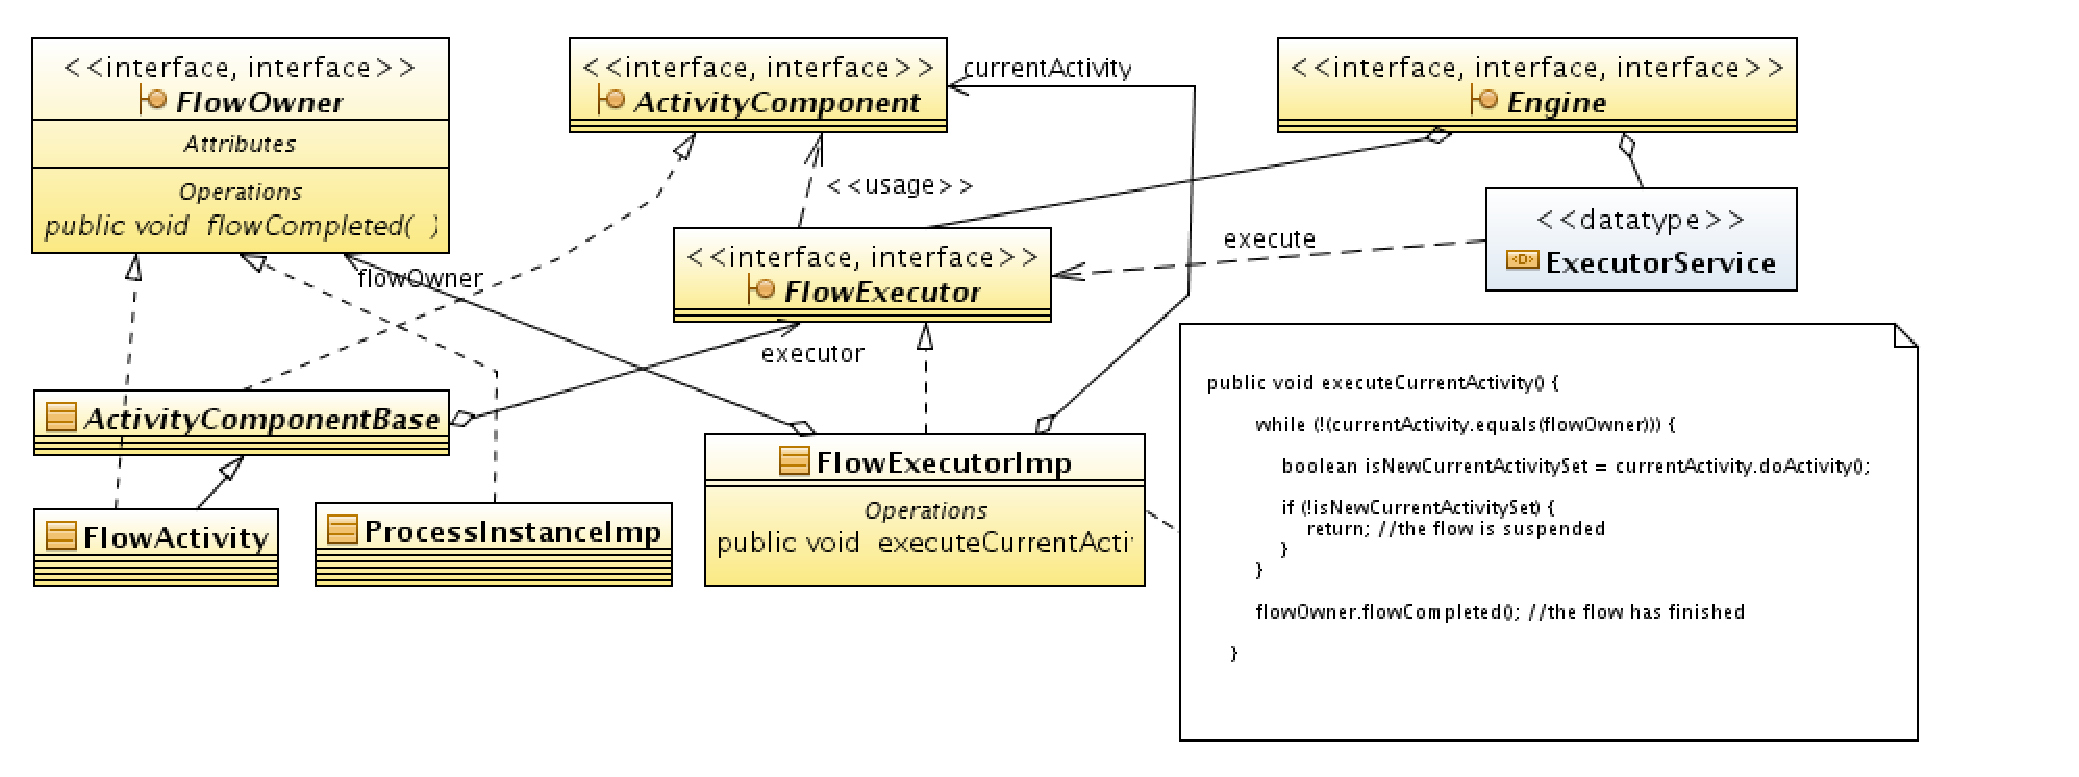
\includegraphics[angle=90,scale=0.75]
{architettura_interna/dia/flowClassDiagram}
\caption[Diagramma di classe FlowExecutor \ldots] {
   	\textsf{{\small Diagramma di classe FlowExecutor, FlowOwner e ThreadPool}} }
  \label{fig:flowclass}
\end{center}
\end{figure}

% %%%%%%%%%%%%%%%%%%%%%%%%%%%%%%%%%%%%%%%%%%%%%%%%%%%%%%%%%%%%%%%%%%%%%%%%%%%%%%%
% EVENTI E COMUNICAZIONE
% %%%%%%%%%%%%%%%%%%%%%%%%%%%%%%%%%%%%%%%%%%%%%%%%%%%%%%%%%%%%%%%%%%%%%%%%%%%%%%%
\section{Comunicazione ed eventi}
Da quanto abbiamo già esposto risulta chiaro che l'esecuzione di un processo \`e
caratterizzata da lo svolgersi di attività interne e l'accadere di eventi
esterni di cui l'attività possono essere in attesa. In generale si può
considerare che gli eventi si generino a livello di Enviroment, e che possano
essere prodotti dall'arrivo di nuovi messaggi verso alle porte locali o
dalla notifica degli acknologment delle invocazioni locali
verso porte remote. Attualmente le funzionalita' espresse da Blite non
individuano eventi diversi da queste due tipologie. Nelle engine pero' si \`e
preferito realizzare un meccanismo generico di notifica di eventi che
soddisfacesse i requisiti attuali del linguaggio ma che non escludesse eventuali
possibilità di estensione verso altre caratteristiche tipiche di BPEL
(comunicazione Request-Response, EventActivity, ecc).

Per l'implementazione dello schema di comunicazione prescelto saranno richieste
le seguenti funzionalita'

\begin{enumerate}
  \item A livello di attività o di ProcessManager stesso,
  sarà necessario ricavare una chiave univoca per uno specifico 
  evento\footnote{Si usa qui il termine ricavare e non generare in maniera
  voluta. Le chiavi di evento non sono identificati da oggetti in memoria ma hanno una loro 
  entità indipendente
  dagli oggetti che posso essere creati per rappresentarle. Per un esempio le
  chiavi utilizzate per la ricezione saranno costituite dalla coppia
  nomeservizio/nomeoperazione, tele coppia verrà indicata come
  \texttt{portId} }. I tipi di evento e le regole per generare di volta in volta 
  le chiavi verranno esposti di seguito. Per il momento può bastare aver
  chiaro che una chiave individua in maniera univoca una particolare tipologia di evento e all'interno di questa un evento specifico o un insieme
  di eventi gemelli. 
  
  \item In un qualsiasi momento al ProcessManager potranno essere notificati
  eventi. In tal caso esso dovrà provvedere a ricavarsi la chiave e a
  memorizzare associativamente l'evento alla chiave per poterlo poi rendere
  disponibile all'attivita' interessate. Il ProcessManager dovrà anche
  provvedere a ``risvegliare'' tutti i flussi di esecuzione che
  eventualmente si sono messi in attesa di quel evento specifico.
   
  \item In un qualsiasi momento e anche più volte nel suo ciclo di vita una
  Attività potrà interrogare l'Engine (o meglio il ProcessManager responsabile
  della sua istanza) chiedendogli se un evento associato ad una particolare
  chiave sia avvenuto. In caso affermativo l'attività potrà consumare l'evento.

  \item Una attività potrà avere la necessità di mettersi in attesa di un
  particolare evento non ancora avvenuto, il tal caso dovrà sospendere il
  suo flusso di esecuzione e notificare questo al ProcessManager
  associativamente alla chiave dell'evento d'interesse. 
\end{enumerate}

Tali funzionalità serrano rese disponibili nelle diverse interfacce 


\ldots
\\

In particolare si può vedere come queste funzionalità di base possano essere
utilizzate nel caso dell'attività \icode{ReceiveActivity}, e come
l'attività stessa collabori con il ProcessManager perché si realizzi la
ricezione di messaggi. La \icode{ReceiveActivity} nel suo metoto doActivity
compiera' i seguenti passi logici:

\begin{enumerate}
  \item Si ricava la chaive d'evento \texttt{eventKey}. In questo caso
  particolare la chiave sara' di tipo \icode{RequestInComingEventKey} e la sua
  unicita' sara costituita dal \texttt{portId} ( ovvero la coppia 
  serviceName/operationName) delle porta su cui si sta eseguendo l'operazione di 
  ricezione. Ovviamente la ReceiveActivity potra' ricavare il \texttt{portId}
  dal nodo della definizione sitattica a lei associata.
  
  \item Si richiede al ProcessManager il set degli eventi associati alla
  \texttt{eventKey}. Se non c'e' alcun evento associato si mette in attesa il
  FlowExecutor sull'evento \texttt{eventKey}, si termina ritornando
  \texttt{false}.
  
  \item Si analizza il set degli eventi (che in questo caso possono essere
  identificati con tutti messaggi indirizzati alla porta in questione non
  ancora consumati) per vedere se ce ne possa essere uno indirizzabile alla
  instanza della ReceiveActivity in questione. Questo controllo \`e fatto in
  base alle regole di correlazione. Se un tale messaggio non viene identificato
  si mette in attesa il FlowExecutor sull'evento \texttt{eventKey} e si termina
  ritornando \texttt{false}. 
  
  \item Si \`e individuato un messaggio inviato alla porta e alla istanza in
  questione. Si consuma tale messaggio aggiornando lo stato delle variabili
  conivolte nella ricezione, si imposta la parentComponet come attivita'
  corrente del FlowExecutor si termina ritornando \texttt{true}.
\end{enumerate}

Daltro canto un oggetto ProcessManager nel metodo \icode{manageRequest( 
ServiceIdentifier service, String operation, MessageContainer
messageContainer)}\footnote{Bisogna notare che
l'invocazione di tale metodo sara' scatenata lato Environment, e che la sua
esecuzione avverra' a carico di un Thread allocato a livello stesso di
Environment e logicamente del tutto indipendente dai thread del pool
dell'Engine} eseguira le seguenti operazioni:

\begin{enumerate}
  \item Si verifica che la terna serviceName/operationName/numero parti del
  messaggio identifichi effettivamente una porta valida per la definizione 
  di processo in questione. Se non \`e cosi si notifica una
  situazione di errore all'Enviroment e questo provvedera' ad inviare un NOK al
  processo invocante.
 
 \item Si ricava il RequestInComingEventKey \texttt{eventKey} associata alla
 porta e con questa si provvede a memorizzare il messaggio in arrivo in una mappa associativa.
 
 \item Se la porta in questione individua una start activity si crea una nuova
 istanza di processo e la si mette in esecuzione, alternativamente 
 
 \item Se la porta non \`e associata ad una start activity si risvegliano tutti
 i FlowExecutor in attesa di eventi individuati dalla \texttt{eventKey}.
\end{enumerate}

Gia' pensando che le due procedure precedenti saranno eseguite concorrentemente
si capisce che un punto particolarmente critico del meccanismo di
notifica/consumo di eventi sta nel fatto che l'elevato grado di parrallelismo
presente possa portare ad una perdita eventi (ovvero non consegna di messaggi).
Quest'ultima \`e di fatto un ipotesi assolutamente inammisibile e che deve essere
assolutamente evitata. Di fatto essa si manifesterebbe allorche il parallelismo
delle fosse sequenzializzato per esempio nel seguente modo

\begin{itemize}
  \item L'\icode{ReceiveActivity} arriva ad eseguire meta' del passo 2. Cioe'
  ricerca eventi non trovandoli ma non arriva a registrare il FlowExecutor come
  in attesa dell'evento.
  \item Il controllo passa al ProcessManager a cui viene effettivamente
  notificato l'evento di interesse della attivita'. Esso pero' non trovando
  nessun FlowExecutor in attesa registra l'eveto e termina.
  \item Il controllo ripassa all'attivita che registra il suo FlowExecutor come
  in attesa. Essendo pero' l'evento gia' accaduto nessuno 
\end{itemize}

% %%%%%%%%%%%%%%%%%%%%%%%%%%%%%%%%%%%%%%%%%%%%%%%%%%%%%%%%%%%%%%%%%%%%%%%%%%%%%%%
% CONTESTI E COMPESAZIONE
% %%%%%%%%%%%%%%%%%%%%%%%%%%%%%%%%%%%%%%%%%%%%%%%%%%%%%%%%%%%%%%%%%%%%%%%%%%%%%%%
\section{Contesti, FaultHandler e Compensazione}



